\documentclass[a4paper]{slides}

\usepackage{tikz}
\usepackage{geometry}
\usepackage{multicol}

\usepackage[scaled]{helvet}
\usepackage[T1]{fontenc}

% Set Layout
\geometry{
    a4paper,
    left=25mm,
    right=25mm,
    top=25mm,
    bottom=25mm
}

\begin{document}

\begin{multicols}{2}

    \fontsize{12}{1}
    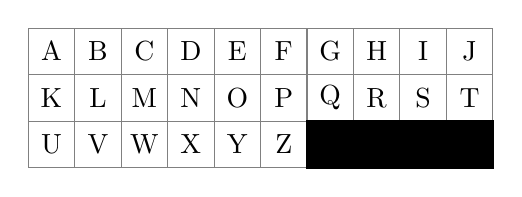
\begin{tikzpicture}[thick, scale=0.59]
        \draw[step=1cm,gray,thin] (0,0) grid (10,3);
        % letter
        \node[anchor = center] () at (0.5,2.5){A};
        \node[anchor = center] () at (1.5,2.5){B};
        \node[anchor = center] () at (2.5,2.5){C};
        \node[anchor = center] () at (3.5,2.5){D};
        \node[anchor = center] () at (4.5,2.5){E};
        \node[anchor = center] () at (5.5,2.5){F};
        \node[anchor = center] () at (6.5,2.5){G};
        \node[anchor = center] () at (7.5,2.5){H};
        \node[anchor = center] () at (8.5,2.5){I};
        \node[anchor = center] () at (9.5,2.5){J};
        \node[anchor = center] () at (0.5,1.5){K};
        \node[anchor = center] () at (1.5,1.5){L};
        \node[anchor = center] () at (2.5,1.5){M};
        \node[anchor = center] () at (3.5,1.5){N};
        \node[anchor = center] () at (4.5,1.5){O};
        \node[anchor = center] () at (5.5,1.5){P};
        \node[anchor = center] () at (6.5,1.5){Q};
        \node[anchor = center] () at (7.5,1.5){R};
        \node[anchor = center] () at (8.5,1.5){S};
        \node[anchor = center] () at (9.5,1.5){T};
        \node[anchor = center] () at (0.5,0.5){U};
        \node[anchor = center] () at (1.5,0.5){V};
        \node[anchor = center] () at (2.5,0.5){W};
        \node[anchor = center] () at (3.5,0.5){X};
        \node[anchor = center] () at (4.5,0.5){Y};
        \node[anchor = center] () at (5.5,0.5){Z};

        % black square
        \filldraw[fill=black, draw=black] (6,0) rectangle (7,1);
        \filldraw[fill=black, draw=black] (7,0) rectangle (8,1);
        \filldraw[fill=black, draw=black] (8,0) rectangle (9,1);
        \filldraw[fill=black, draw=black] (9,0) rectangle (10,1);
    \end{tikzpicture}

    \fontsize{12}{1}
    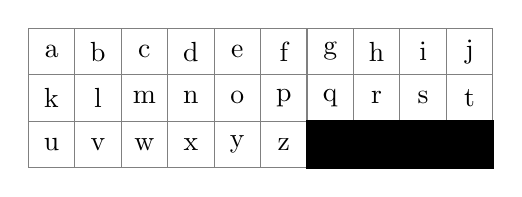
\begin{tikzpicture}[thick, scale=0.59]
        \draw[step=1cm,gray,thin] (0,0) grid (10,3);
        % letter
        \node[anchor = center] () at (0.5,2.5){a};
        \node[anchor = center] () at (1.5,2.5){b};
        \node[anchor = center] () at (2.5,2.5){c};
        \node[anchor = center] () at (3.5,2.5){d};
        \node[anchor = center] () at (4.5,2.5){e};
        \node[anchor = center] () at (5.5,2.5){f};
        \node[anchor = center] () at (6.5,2.5){g};
        \node[anchor = center] () at (7.5,2.5){h};
        \node[anchor = center] () at (8.5,2.5){i};
        \node[anchor = center] () at (9.5,2.5){j};
        \node[anchor = center] () at (0.5,1.5){k};
        \node[anchor = center] () at (1.5,1.5){l};
        \node[anchor = center] () at (2.5,1.5){m};
        \node[anchor = center] () at (3.5,1.5){n};
        \node[anchor = center] () at (4.5,1.5){o};
        \node[anchor = center] () at (5.5,1.5){p};
        \node[anchor = center] () at (6.5,1.5){q};
        \node[anchor = center] () at (7.5,1.5){r};
        \node[anchor = center] () at (8.5,1.5){s};
        \node[anchor = center] () at (9.5,1.5){t};
        \node[anchor = center] () at (0.5,0.5){u};
        \node[anchor = center] () at (1.5,0.5){v};
        \node[anchor = center] () at (2.5,0.5){w};
        \node[anchor = center] () at (3.5,0.5){x};
        \node[anchor = center] () at (4.5,0.5){y};
        \node[anchor = center] () at (5.5,0.5){z};

        % black square
        \filldraw[fill=black, draw=black] (6,0) rectangle (7,1);
        \filldraw[fill=black, draw=black] (7,0) rectangle (8,1);
        \filldraw[fill=black, draw=black] (8,0) rectangle (9,1);
        \filldraw[fill=black, draw=black] (9,0) rectangle (10,1);
    \end{tikzpicture}

\end{multicols}


\fontsize{14}{1.5}\textbf{Bitte Großbuchstaben in Schreibrichtung eintragen}

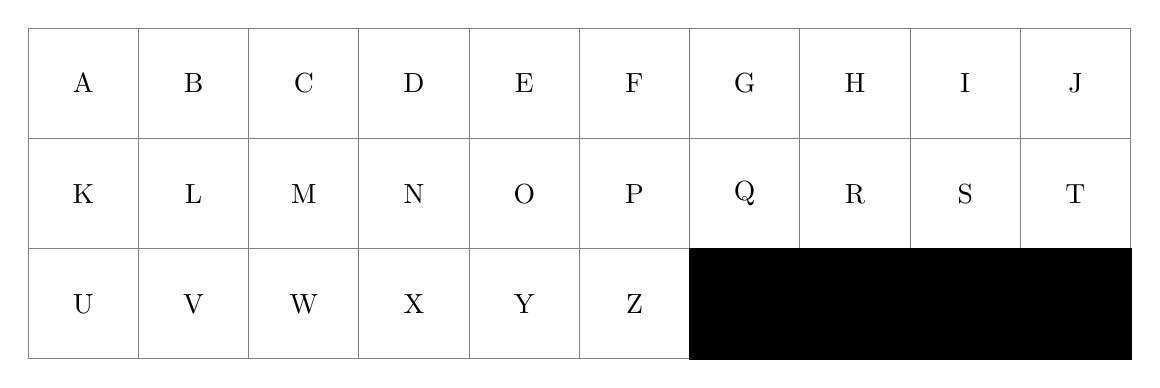
\begin{tikzpicture}[thick, scale=1.4]
    \draw[step=1cm,gray,thin] (0,0) grid (10,3);
    % letters
    \node[anchor = center] () at (0.5,2.5){A};
    \node[anchor = center] () at (1.5,2.5){B};
    \node[anchor = center] () at (2.5,2.5){C};
    \node[anchor = center] () at (3.5,2.5){D};
    \node[anchor = center] () at (4.5,2.5){E};
    \node[anchor = center] () at (5.5,2.5){F};
    \node[anchor = center] () at (6.5,2.5){G};
    \node[anchor = center] () at (7.5,2.5){H};
    \node[anchor = center] () at (8.5,2.5){I};
    \node[anchor = center] () at (9.5,2.5){J};
    \node[anchor = center] () at (0.5,1.5){K};
    \node[anchor = center] () at (1.5,1.5){L};
    \node[anchor = center] () at (2.5,1.5){M};
    \node[anchor = center] () at (3.5,1.5){N};
    \node[anchor = center] () at (4.5,1.5){O};
    \node[anchor = center] () at (5.5,1.5){P};
    \node[anchor = center] () at (6.5,1.5){Q};
    \node[anchor = center] () at (7.5,1.5){R};
    \node[anchor = center] () at (8.5,1.5){S};
    \node[anchor = center] () at (9.5,1.5){T};
    \node[anchor = center] () at (0.5,0.5){U};
    \node[anchor = center] () at (1.5,0.5){V};
    \node[anchor = center] () at (2.5,0.5){W};
    \node[anchor = center] () at (3.5,0.5){X};
    \node[anchor = center] () at (4.5,0.5){Y};
    \node[anchor = center] () at (5.5,0.5){Z};

    % black square
    \filldraw[fill=black, draw=black] (6,0) rectangle (7,1);
    \filldraw[fill=black, draw=black] (7,0) rectangle (8,1);
    \filldraw[fill=black, draw=black] (8,0) rectangle (9,1);
    \filldraw[fill=black, draw=black] (9,0) rectangle (10,1); 
\end{tikzpicture}

\fontsize{14}{1.5}\textbf{Bitte Kleinbuchstaben in Schreibrichtung Eintragen}

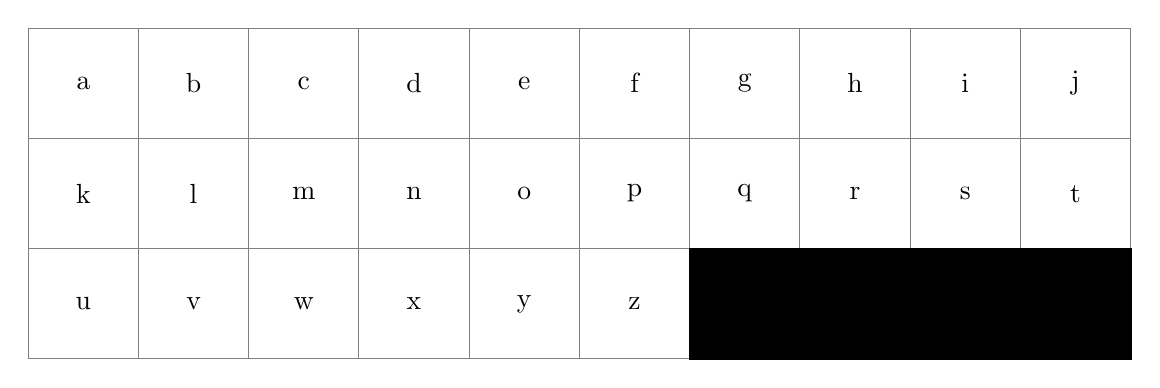
\begin{tikzpicture}[thick, scale=1.4]
    \draw[step=1cm,gray,thin] (0,0) grid (10,3);
    % letter
    \node[anchor = center] () at (0.5,2.5){a};
    \node[anchor = center] () at (1.5,2.5){b};
    \node[anchor = center] () at (2.5,2.5){c};
    \node[anchor = center] () at (3.5,2.5){d};
    \node[anchor = center] () at (4.5,2.5){e};
    \node[anchor = center] () at (5.5,2.5){f};
    \node[anchor = center] () at (6.5,2.5){g};
    \node[anchor = center] () at (7.5,2.5){h};
    \node[anchor = center] () at (8.5,2.5){i};
    \node[anchor = center] () at (9.5,2.5){j};
    \node[anchor = center] () at (0.5,1.5){k};
    \node[anchor = center] () at (1.5,1.5){l};
    \node[anchor = center] () at (2.5,1.5){m};
    \node[anchor = center] () at (3.5,1.5){n};
    \node[anchor = center] () at (4.5,1.5){o};
    \node[anchor = center] () at (5.5,1.5){p};
    \node[anchor = center] () at (6.5,1.5){q};
    \node[anchor = center] () at (7.5,1.5){r};
    \node[anchor = center] () at (8.5,1.5){s};
    \node[anchor = center] () at (9.5,1.5){t};
    \node[anchor = center] () at (0.5,0.5){u};
    \node[anchor = center] () at (1.5,0.5){v};
    \node[anchor = center] () at (2.5,0.5){w};
    \node[anchor = center] () at (3.5,0.5){x};
    \node[anchor = center] () at (4.5,0.5){y};
    \node[anchor = center] () at (5.5,0.5){z};

    % black square
    \filldraw[fill=black, draw=black] (6,0) rectangle (7,1);
    \filldraw[fill=black, draw=black] (7,0) rectangle (8,1);
    \filldraw[fill=black, draw=black] (8,0) rectangle (9,1);
    \filldraw[fill=black, draw=black] (9,0) rectangle (10,1);
\end{tikzpicture}

\fontsize{14}{1.5}\textbf{Bitte in jede Reihe die Zahlen von 0 bis 9 eintragen }

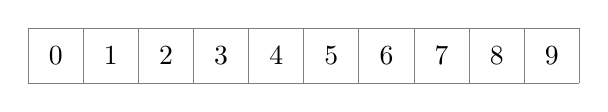
\begin{tikzpicture}[thick, scale=0.7]
    \draw[step=1cm,gray,thin] (0,0) grid (10,1);
    \node[anchor = center] () at (0.5,0.5){0};
    \node[anchor = center] () at (1.5,0.5){1};
    \node[anchor = center] () at (2.5,0.5){2};
    \node[anchor = center] () at (3.5,0.5){3};
    \node[anchor = center] () at (4.5,0.5){4};
    \node[anchor = center] () at (5.5,0.5){5};
    \node[anchor = center] () at (6.5,0.5){6};
    \node[anchor = center] () at (7.5,0.5){7};
    \node[anchor = center] () at (8.5,0.5){8};
    \node[anchor = center] () at (9.5,0.5){9};
\end{tikzpicture}

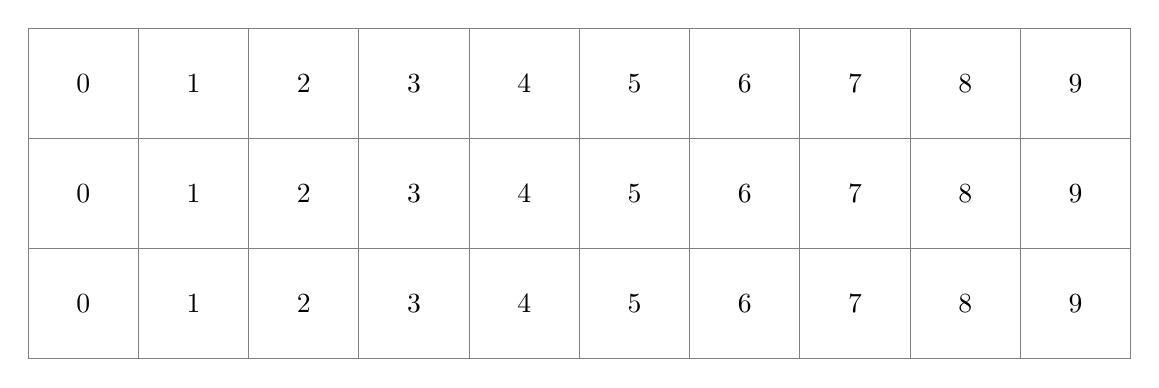
\begin{tikzpicture}[thick, scale=1.4]
    \draw[step=1cm,gray,thin] (0,0) grid (10,3);
    \node[anchor = center] () at (0.5,0.5){0};
    \node[anchor = center] () at (1.5,0.5){1};
    \node[anchor = center] () at (2.5,0.5){2};
    \node[anchor = center] () at (3.5,0.5){3};
    \node[anchor = center] () at (4.5,0.5){4};
    \node[anchor = center] () at (5.5,0.5){5};
    \node[anchor = center] () at (6.5,0.5){6};
    \node[anchor = center] () at (7.5,0.5){7};
    \node[anchor = center] () at (8.5,0.5){8};
    \node[anchor = center] () at (9.5,0.5){9};
    
    \node[anchor = center] () at (0.5,1.5){0};
    \node[anchor = center] () at (1.5,1.5){1};
    \node[anchor = center] () at (2.5,1.5){2};
    \node[anchor = center] () at (3.5,1.5){3};
    \node[anchor = center] () at (4.5,1.5){4};
    \node[anchor = center] () at (5.5,1.5){5};
    \node[anchor = center] () at (6.5,1.5){6};
    \node[anchor = center] () at (7.5,1.5){7};
    \node[anchor = center] () at (8.5,1.5){8};
    \node[anchor = center] () at (9.5,1.5){9};

    \node[anchor = center] () at (0.5,2.5){0};
    \node[anchor = center] () at (1.5,2.5){1};
    \node[anchor = center] () at (2.5,2.5){2};
    \node[anchor = center] () at (3.5,2.5){3};
    \node[anchor = center] () at (4.5,2.5){4};
    \node[anchor = center] () at (5.5,2.5){5};
    \node[anchor = center] () at (6.5,2.5){6};
    \node[anchor = center] () at (7.5,2.5){7};
    \node[anchor = center] () at (8.5,2.5){8};
    \node[anchor = center] () at (9.5,2.5){9};
\end{tikzpicture}

\end{document}
